\begin{frame}{Training specifications}
  \begin{itemize}
      \item Training a deep neural network
      \vspace{0.2cm}
      \item Coarse optimisation using an evolutionary neural network
      \vspace{0.2cm}
      \item Fine optimisation doing a grid search
      \vspace{0.2cm}
      \item Optimised hyperparameters:
          \begin{itemize}
              \item Number of nodes
              \item Number of layers
              \item Dropout percentage
              \item Activation function
              \item Weight initialisation
              \item Optimiser
          \end{itemize}
      \item Signal: tHq, tZq
      \item Background: Diboson, Z+jets, ttbar
      \item Using absolute weights
  \end{itemize}
\end{frame}

\begin{frame}{Evolutionary optimisation of neural networks}
    \begin{itemize}
        \item Combination of a grid searches with a survival of the fittest setup
        \vspace{0.2cm}
        \item Start with a number of random hyperparamters
        \vspace{0.2cm}
        \item Evaluate the set of hyperparameters
        \vspace{0.2cm}
        \item Create a a new set of networks based on the previous best
        \vspace{0.2cm}
        \item Add recombination and variation to avoid local minima and bias
    \end{itemize}
\end{frame}



\begin{frame}{Setup}
    \begin{itemize}
        \item \tZq as signal against \ttbar as background
        \item Using basic kinematic variables
        \item No specific region
        \item Training without weights due to some recent problems
        \item Testing: nodes, layers, dropout
        \item Fixed hyperparameters:
            \begin{itemize}
                \item Optimizer: Adam
                \item Activation: relu, sigmoid
                \item Batchsize: 1000
                \item Epochs: 25
            \end{itemize}
    \end{itemize}
\end{frame}

\begin{frame}{An example of parameter development}
     \begin{block}{Initial parameters}
         \begin{itemize}
             \item Layers: $1-10$
             \item Nodes: $1-100$
             \item Dropout: $0-1$
         \end{itemize}
     \end{block}
     \begin{block}{Final parameters}
         \begin{itemize}
             \item Layers: $4\pm2$
             \item Nodes: $67\pm33$
             \item Dropout: $0.4\pm0.3$
         \end{itemize}
     \end{block}
\end{frame}

%\begin{frame}{ROC and Separation}
%    \begin{columns}
%        \begin{column}{0.5\textwidth}
%            \begin{figure}
%                \centering
%                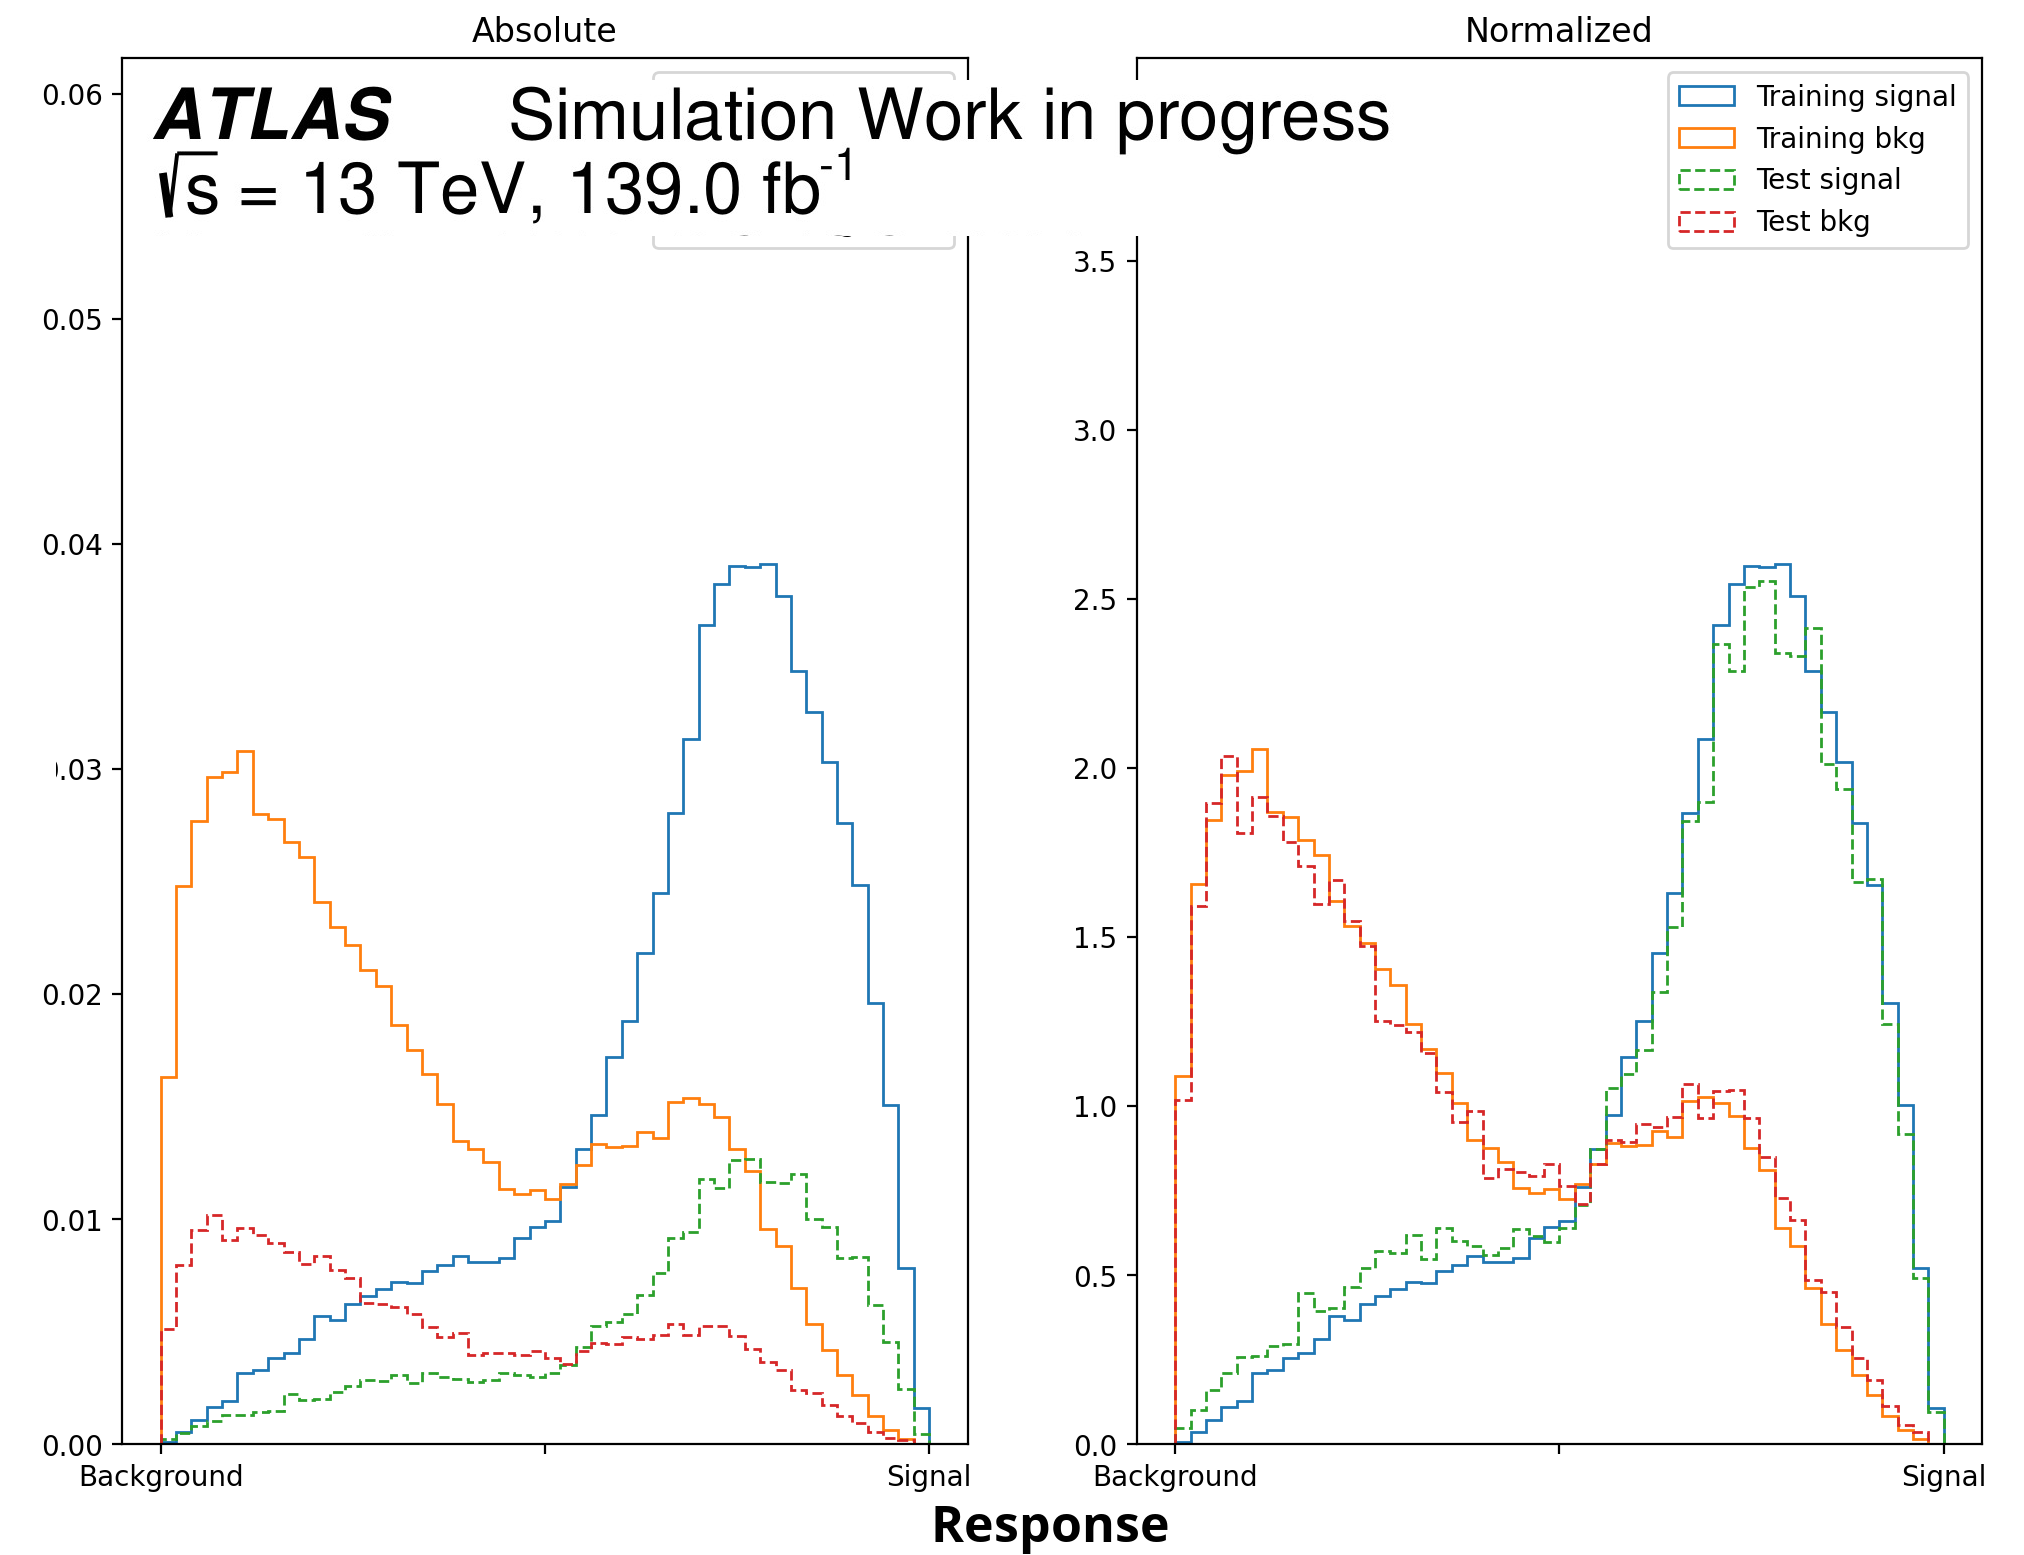
\includegraphics[width = \textwidth]{evo_response.png}
%            \end{figure}
%        \end{column}
%        \begin{column}{0.5\textwidth}
%            \begin{figure}
%                \centering
%                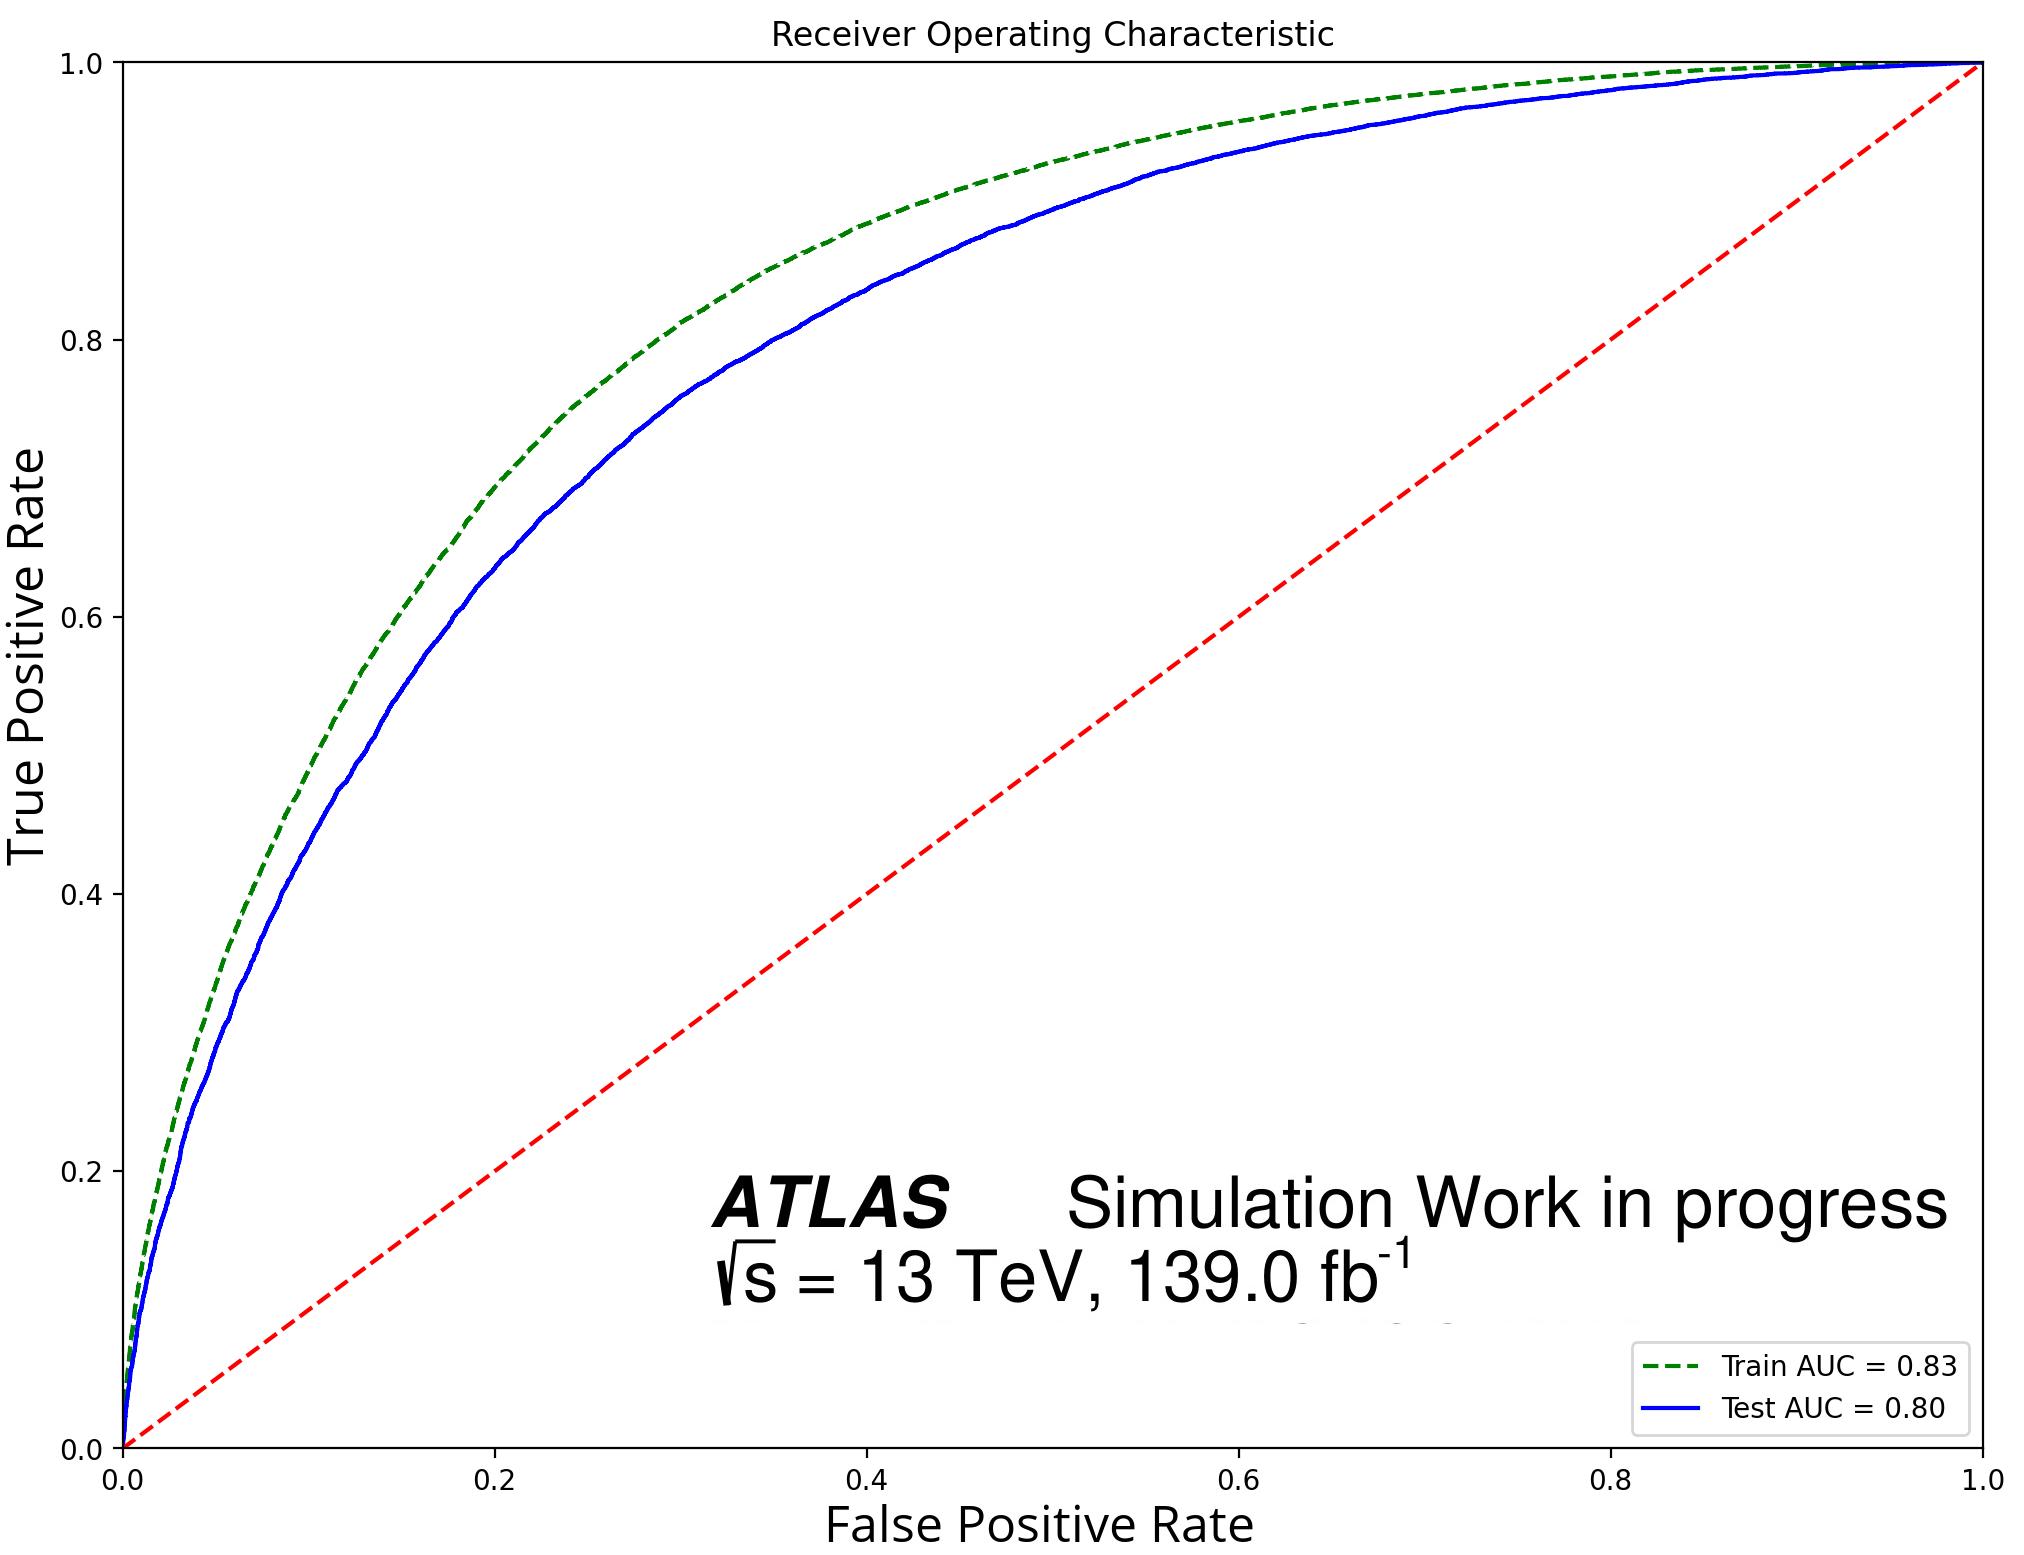
\includegraphics[width = \textwidth]{evo_ROC.png}
%            \end{figure}
%        \end{column}
%    \end{columns}
%\end{frame}

\begin{frame}{Comparing to a grid search}
    \begin{columns}
        \begin{column}{0.5\textwidth}
            \begin{figure}
                \centering
                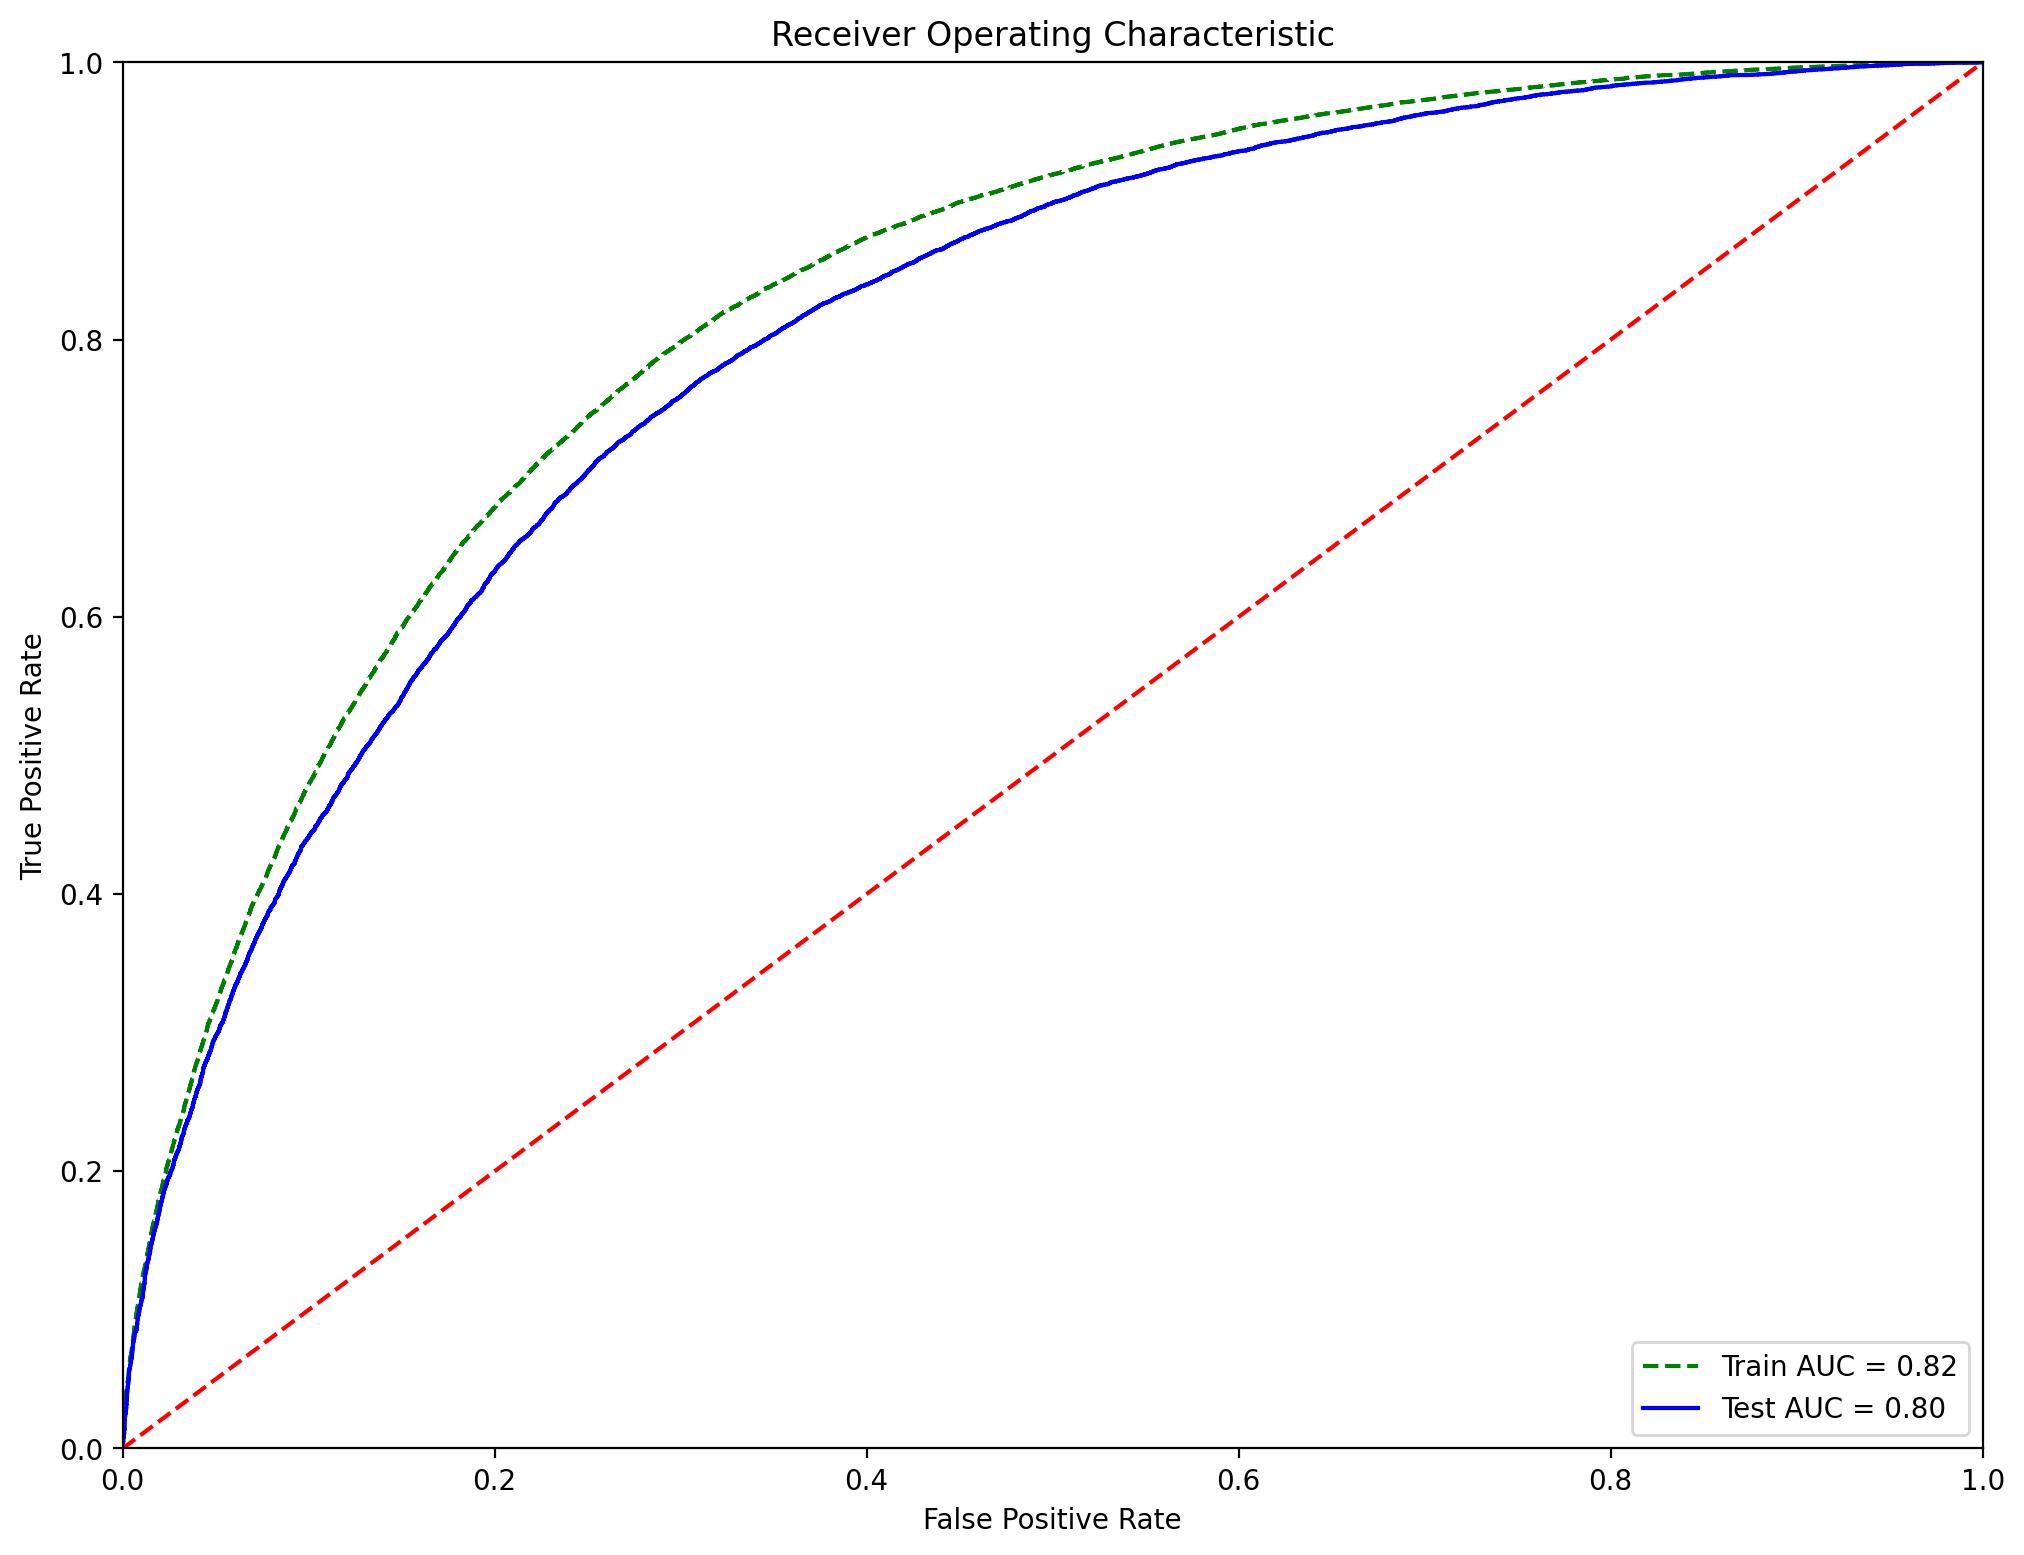
\includegraphics[width = \textwidth]{grid_ROC.png}
                \caption{Grid search}
            \end{figure}
        \end{column}
        \begin{column}{0.5\textwidth}
            \begin{figure}
                \centering
                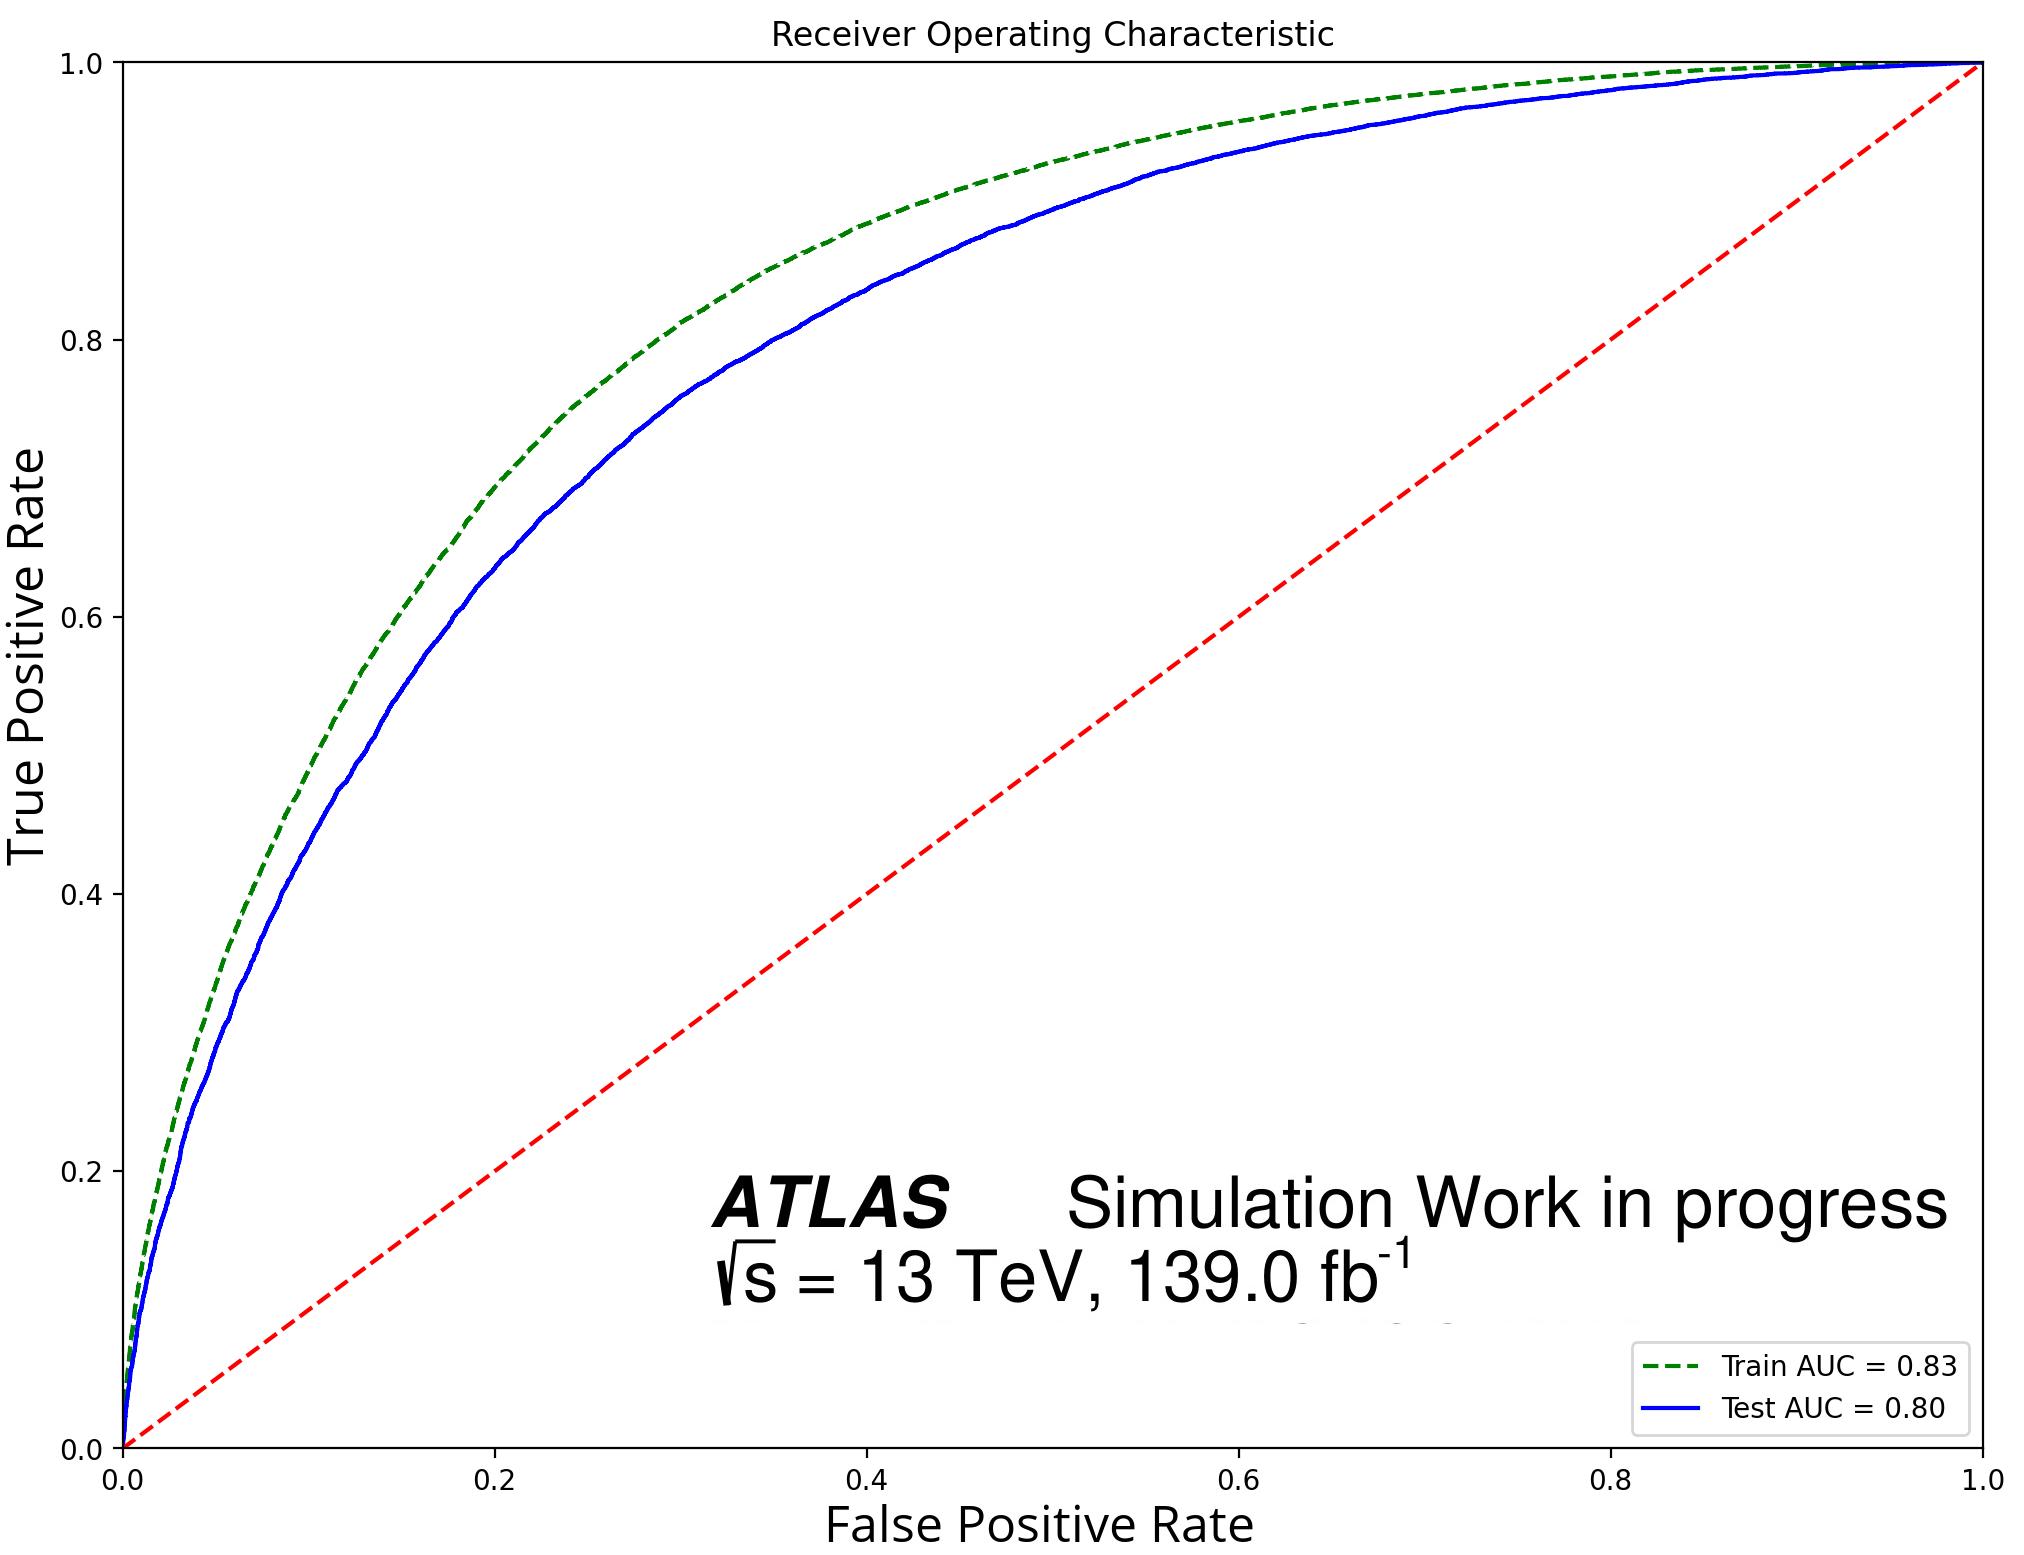
\includegraphics[width = \textwidth]{evo_ROC.png}
                \caption{Evolutionary search}
            \end{figure}
        \end{column}
    \end{columns}
\end{frame}


\begin{frame}{Comparing to a grid search}
    \begin{columns}
        \begin{column}{0.5\textwidth}
            \begin{figure}
                \centering
                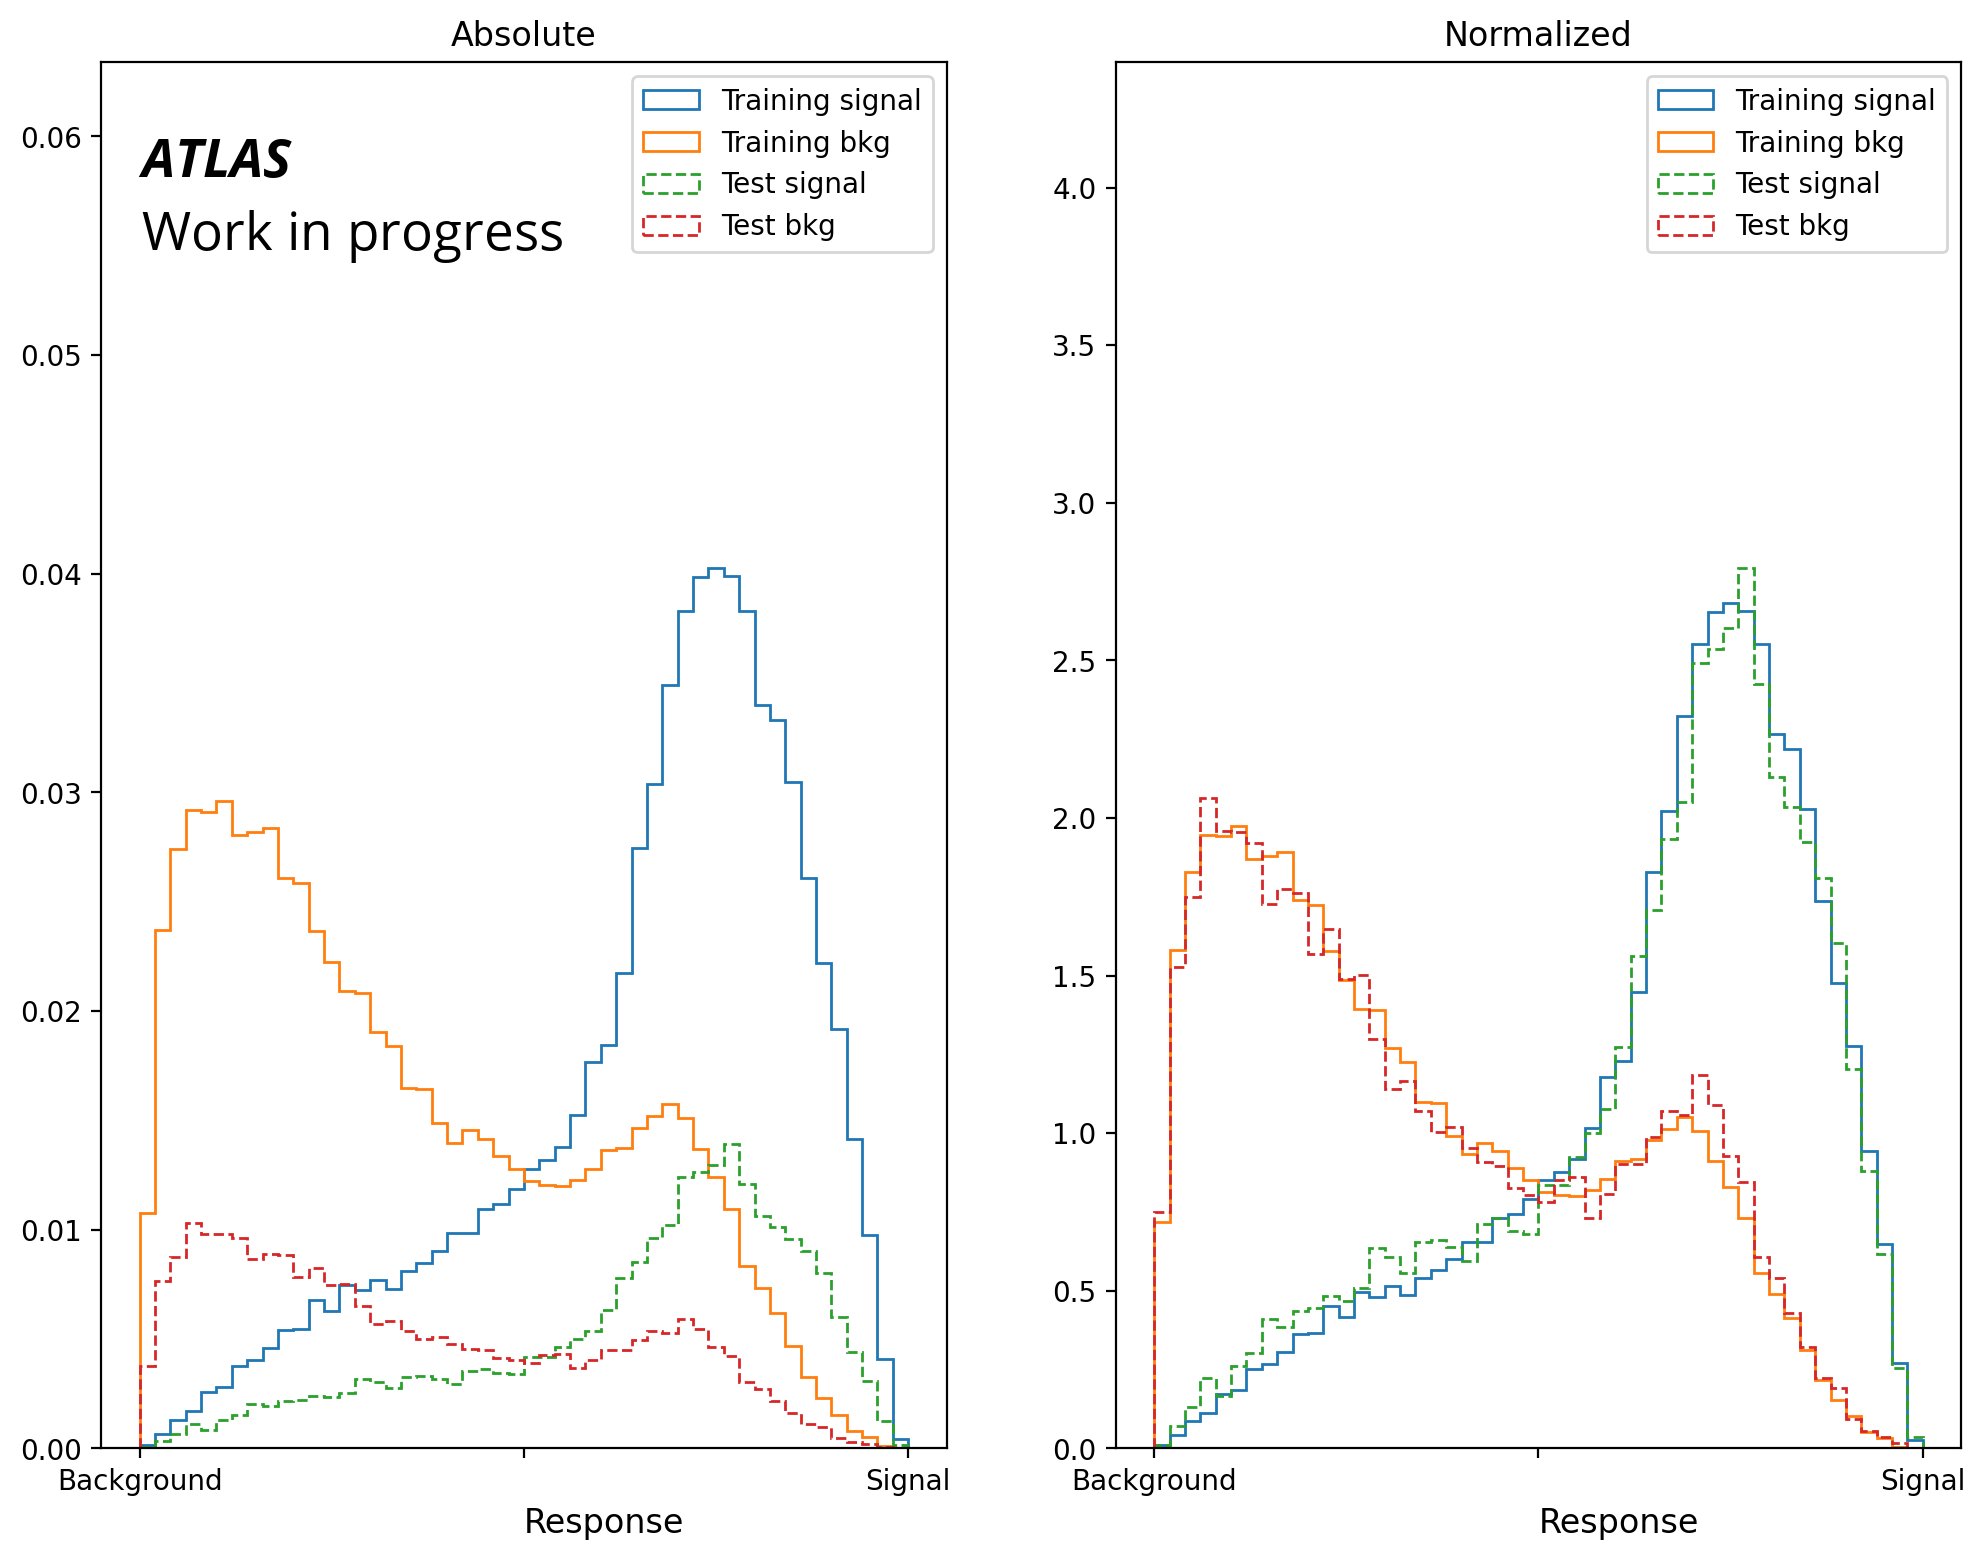
\includegraphics[width = \textwidth]{grid_response.png}
                \caption{Grid search}
            \end{figure}
        \end{column}
        \begin{column}{0.5\textwidth}
            \begin{figure}
                \centering
                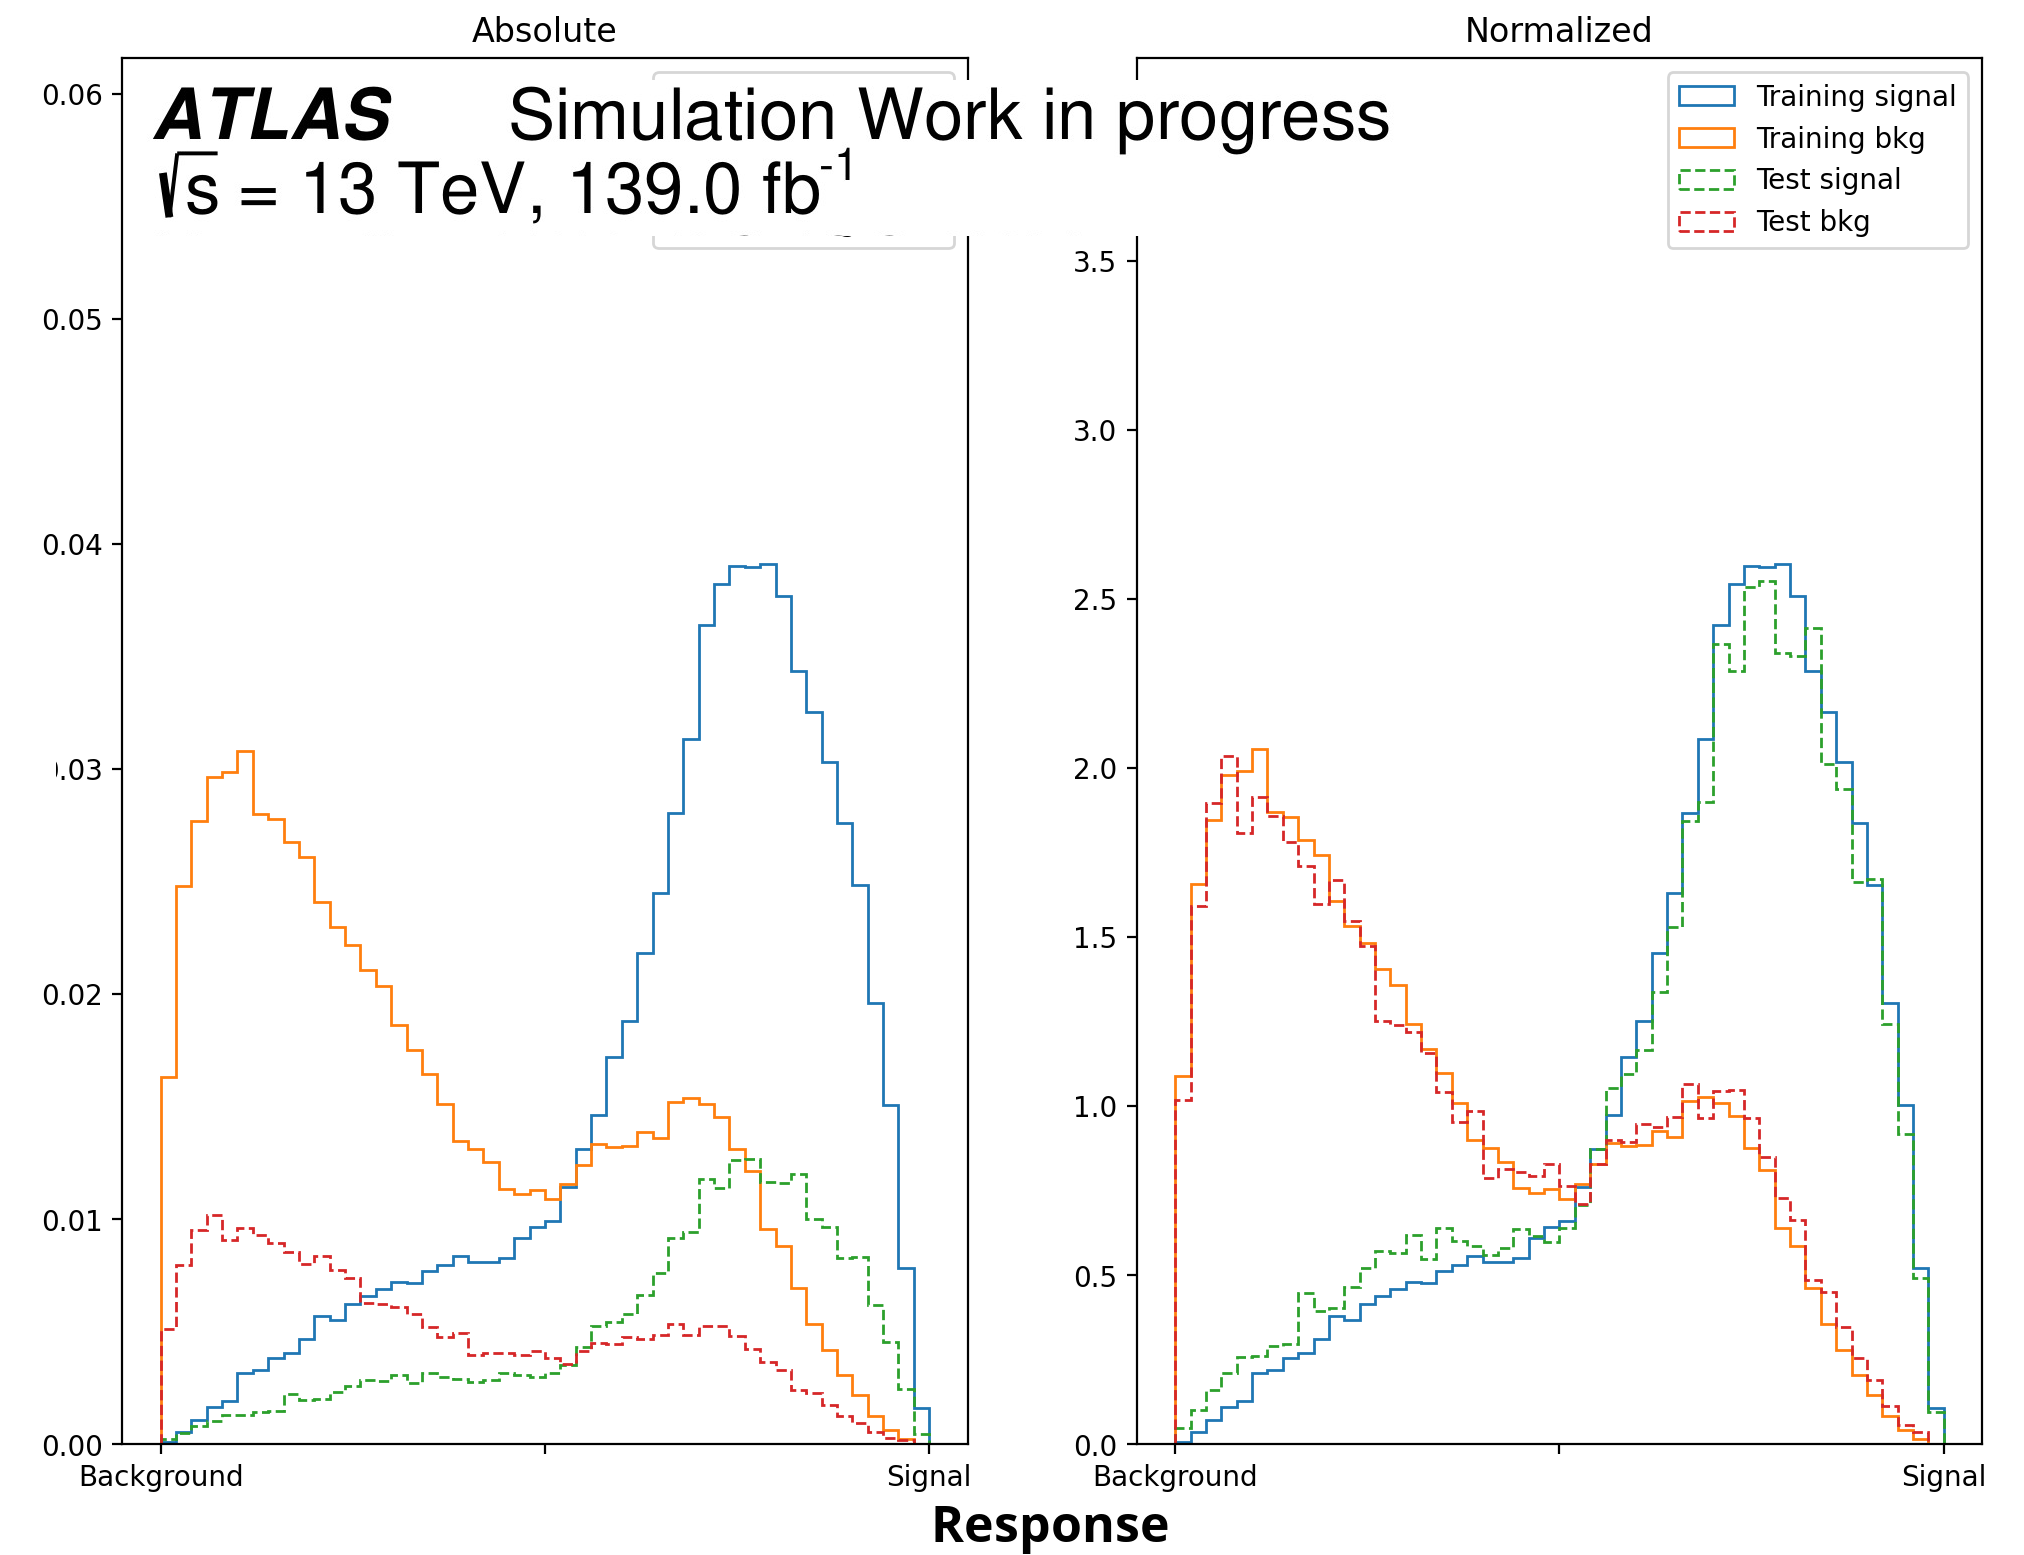
\includegraphics[width = \textwidth]{evo_response.png}
                \caption{Evolutionary search}
            \end{figure}
        \end{column}
    \end{columns}
\end{frame}